\documentclass[12pt]{article}
\usepackage[top=1in, bottom=1in, left=1in, right=1in]{geometry}

\usepackage{setspace}
\onehalfspacing

\usepackage{amssymb}
%% The amsthm package provides extended theorem environments
\usepackage{amsthm}
\usepackage{epsfig}
\usepackage{times}
\renewcommand{\ttdefault}{cmtt}
\usepackage{amsmath}
\usepackage{graphicx} % for graphics files

% Draw figures yourself
\usepackage{tikz} 

% writing elements
\usepackage{mhchem}

% The float package HAS to load before hyperref
\usepackage{float} % for psuedocode formatting
\usepackage{xspace}

% from Denovo Methods Manual
\usepackage{mathrsfs}
\usepackage[mathcal]{euscript}
\usepackage{color}
\usepackage{array}

\usepackage[pdftex]{hyperref}
\usepackage[parfill]{parskip}

% math syntax
\newcommand{\nth}{n\ensuremath{^{\text{th}}} }
\newcommand{\ve}[1]{\ensuremath{\mathbf{#1}}}
\newcommand{\Macro}{\ensuremath{\Sigma}}
\newcommand{\rvec}{\ensuremath{\vec{r}}}
\newcommand{\vecr}{\ensuremath{\vec{r}}}
\newcommand{\omvec}{\ensuremath{\hat{\Omega}}}
\newcommand{\vOmega}{\ensuremath{\hat{\Omega}}}
\newcommand{\sigs}{\ensuremath{\Sigma_s(\rvec,E'\rightarrow E,\omvec'\rightarrow\omvec)}}
\newcommand{\el}{\ensuremath{\ell}}
\newcommand{\sigso}{\ensuremath{\Sigma_{s,0}}}
\newcommand{\sigsi}{\ensuremath{\Sigma_{s,1}}}
%---------------------------------------------------------------------------
%---------------------------------------------------------------------------
\begin{document}
\begin{center}
{\bf NE 250, F15\\
October 12, 2015 
}
\end{center}

Last time we derived the integral form of the TE:
\begin{equation}
\psi(\rvec, \vOmega, E) =\int_0^{\infty} d\rho' \:\exp[-\int_0^{\rho'} d\rho'' \: \Sigma_t(\rvec-\rho''\vOmega,E)]q(\rvec-\rho'\vOmega,\vOmega,E)
\label{eq:integral}
\end{equation}
%
We can reframe with with operators to think about how the levels of collisions build up the flux at a given point in phase space.\\
If we define $Q'$ as the integrated fixed source and\\
$K$ as the appropriate integral operator \\
then $K\psi$ is the neutron production by scattering and fission. \\
We can then see
\[\psi = K \psi + Q'\]
We can think about this equation 
\begin{align*}
\psi_0 &= Q' \quad \text{uncollided flux}\\
\psi_1 &= K \psi_0 \quad \text{flux of neutrons that have had one collision}\\
&\vdots \\
\psi_n &= K \psi_{n-1} \quad \text{flux of neutrons that have had n collisions} \\
\psi &= \sum_{j=0}^{\infty} \psi_j \quad \text{total flux distribution}
\end{align*}

---------------------------\\
If we have \textbf{isotropic scattering} and \textbf{isotropic sources}, we can remove the angle dependence and up with a volume integral.
%
\begin{itemize}
\item The fission process is isotropic:
\[\frac{\chi(E)}{4\pi} \int_0^{\infty} dE' \: \nu(E') \Sigma_f(\rvec, E') \underbrace{\int_{4\pi} d\vOmega' \: \psi(\rvec, \vOmega', E')}_{\phi(\rvec,E')}\]
\item The fixed source becomes
\[S(\rvec, \vOmega, E) = \frac{S(\rvec, E)}{4 \pi}\]
\item and the scattering source becomes
\[\int_0^{\infty} dE' \int_{4\pi} d\vOmega' \: \frac{\Sigma_s(\rvec,E' \rightarrow E)}{4\pi} \psi(\rvec, \vOmega', E') = \frac{1}{4\pi}\int_0^{\infty} dE'\:\Sigma_s(\rvec,E' \rightarrow E) \phi(\rvec,E')\]
\item The total source is the sum of these three, and is now independent of angle.
\end{itemize}
%
We can use this source in Eqn.~\ref{eq:integral}, integrate the integrating factor over angle, and get an expression for the scalar flux. When doing this, we will note the following things based on the figure below
%
\begin{figure}[h]
\begin{center}
  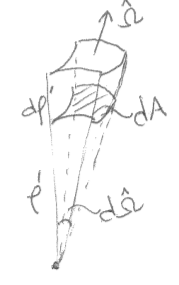
\includegraphics[width=1.25 in]{../figs/diff-area}
\end{center}
\end{figure}
\begin{align*}
d\vOmega &= \frac{dA}{\rho'^2}\\
d\rho' dA &= dV \\
\int_{4\pi} d\vOmega \int_0^{\infty} d\rho' &-= \int_{V} \frac{dV}{\rho'^2}
\end{align*}
%
We can also recall that $\rho' = |\vec{r} - \vec{r}'|$, we can let $dV = d^3r'$, and we will define
\[\int_0^{\rho'} d\rho'' \: \Sigma_t(\rvec-\rho''\vOmega,E) \equiv \tau(E,\vec{r} - \rho' \vOmega \rightarrow \vec{r})
\]
which is the optical path length. \\
Combining all of this we get
\begin{align}
\phi(\rvec,E) &= \int_V d^3r' \: \biggl[\frac{\exp[-\tau(E,\vec{r}' \rightarrow \vec{r})]}{4\pi|\vec{r} - \vec{r}'|^2} \biggl(S(\vec{r}',E) + \frac{\chi(E)}{4\pi} \int_0^{\infty} dE' \: \nu(E') \Sigma_f(\rvec', E')\phi(\vec{r}', E') \nonumber \\
&+ \int_0^{\infty} dE'\:\Sigma_s(\rvec',E' \rightarrow E) \phi(\rvec',E') \biggr)  \biggr]
\label{eq:iso-integral}
\end{align}
%
Interestingly, if $|\vec{r} - \vec{r}'|$ is replaced by $R$, then in the simple case of total cross section being independent of position, Eqn.~\ref{eq:iso-integral} becomes
\[\phi(\rvec,E) = \int_V d^3r' \: \biggl[\frac{\exp[-\Sigma_t(E, R)]}{4\pi R^2} \biggl( \text{isotropic source at }\vec{r}' \biggr)\biggr]\]

In both of these equations, the source term is the rate at which neutrons of energy $E$ appear at $\vec{r}'$ from each source type. \\
In this last equation, the term multiplying the source is the probability that a neutron appearing at $\vec{r}'$ will reach $\vec{r}$ without suffering a collision.\\
The integration over all values of $\vec{r}'$ is equivalent to adding neutrons from all possible sources. \\
It is of interest to note that the exponential term, including the denominator, is a Green's function for a unit isotropic source at $\vec{r}'$ in an absorbing medium.

---------------------------\\
We frequently, however, have \textbf{anisotopric scattering}. We can derive an equation similar to the isotropic one.\\
We will reframe how we think about the source. We will say the production kernel is
%
\[\Pi(\rvec, \vOmega',E' \rightarrow \vOmega, E) \equiv \Sigma_s(\rvec, \vOmega',E' \rightarrow \vOmega, E) + \frac{\chi(E)}{4\pi} \nu(E') \Sigma_f(\rvec', E')\]
Then, the collision source of neutrons is
\[\Phi(\vec{r}, \vOmega, E) = \int_{4\pi} d\vOmega' \int_0^{\infty} dE' \: \Pi(\rvec, \vOmega',E' \rightarrow \vOmega, E) \psi(\rvec, \vOmega', E')\]
%
We can say that $q$ is the collision source combined with the external source. We perform the same sort of operations as above, and now we have an integral equation that has $\Phi$ as a dependent variable. See B\&G 1.2d for a full treatment.

---------------------------\\
The \textbf{Adjoint Transport Equation} (L\&M 1.6).

The adjoint TE has two main applications: use in MC variance reduction and use in perturbation theory for eigenvalue problems (estimate changes in the neutron multiplication cause by small changes in material properties). \\
We will start with some mathematical concepts we will use.

\textit{Inner product}
\begin{itemize}
\item An inner product is a binary operation (takes 2 arguments) that combines 2 vectors into a scalar quantity.
\item in Euclidean space comprises all 3D vectors the inner product is the project of one vector onto another ($\vec{v}_1 \cdot \vec{v}_2 = |v_1||v_2|\cos(\theta)$).
\item Euclidean space (comprises all 3D vectors)
\item A function space comprises all functions that have a given property. e.g.\ all continuous functions; all functions with Dirichlet BCs; etc.
\item $f \: \in$ a function space: $f$ satisfies the properties of the space
\item one way to define an inner product: $<f,g> \equiv \int_{\rho} d\rho \: f^{*}(\rho) g(\rho)$, where superscript $*$ indicates complex conjugate.
\item Inner products are linear: $<f, [ag_1 + bg_2]> = a<f, g_1> + b<f, g_2>$ ($a$ and $b$ are scalars).
\end{itemize}


\end{document}
